\documentclass[a4paper,10pt]{article}
\usepackage[utf8x]{inputenc}
\usepackage{amsmath}
\usepackage{amsfonts}
\usepackage{relsize}
\usepackage[smaller]{acronym}
\usepackage{graphicx}
\usepackage{subfigure}
\usepackage{cite}
\usepackage{url}
\usepackage{hyperref}
\usepackage{color}

\acrodef{WSN}{Wireless sensor network}
\acrodef{TEG}{Thermoelectric generator}
\acrodef{EH}{Energy harvesting}

%opening
\title{Energy Harvesting}
\author{Author: Miha \v Can\v cula \\ Mentor: doc. dr. Du\v san Ponikvar}

\begin{document}

\maketitle

\begin{abstract}

\end{abstract}

\tableofcontents

\section{Introduction}

Small electronic devices are increasingly present everywhere around us. With their ubiquity and ever decreasing size and power consumption, connecting each of them to the power grid becomes impractical. 

The traditional solution is to use batteries, but they come with their own set of problems. Replacing them can be expensive, especially in hard-to-reach places. A much better option would be if the device had a power source of its own, removing its dependence on the power grid and drastically reducing the maintanace cost~\cite{Burgoine11}. 

The method of drawing small amounts of electricity from the device's immediate surrounding is called \ac{EH}. 

\section{Use-cases}

\subsection{Sensors}

A very common use for energy harvesting systems are nodes in \acp{WSN}~\cite{teg-wsn-ieee,cap-wsn-ieee}. Such a network can contain a large number of independent nodes, so it would be difficult to connect each node to the power grid with wires. The sensors themselves usually consume very small amounts of power, so they are ideal applications for \acl{EH} methods. 

% list is from wikipedia: https://en.wikipedia.org/wiki/Energy_harvesting
The applications for \acp{WSN} include~\cite{wiki:eh}:
\begin{itemize}
  \item Weather stations
  \item Air and water pollution measuring
  \item Fire detection
  \item Industrial machine health monitoring
  \item Structural monitoring in buildings
  \item Intelligent buildings~\cite{cap-wsn-ieee}
\end{itemize}

Most of these applications require the nodes to be outside or in other areas where a direct connection to the grid would be difficult. On the other hand, they can still be close enough to the central node so they can transmit the measurements over a wireless connection with their own harvested power. 

Another important characteristic of sensor nodes is their power consumption profile. Often they will be idle for a long time (from minutes to days), and perform measurements in a relatively short time. The transmission of data can be even more infrequent, depending on whether the data has to be available immediately or not. In any case, sensor nodes consume very little current in the idle time period, with short bursts of consumption at regular intervals. An example of such consumption profile in is Figure~\ref{fig:wsn-consumption}. 

\begin{figure}[h]
\centering
 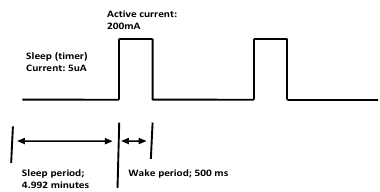
\includegraphics[width=250pt]{./Slike/wsn-current-profile}
 \caption{An example of a \ac{WSN} current consumption profile~\cite{cap-wsn-ieee}}
\label{fig:wsn-consumption}
\end{figure}


\subsection{Consumer electronics}

Many popular electronic devices, including TV remote controls, digital watches, portable music players and mobile phones, have power consumption low enough to be powered or at least assisted by \ac{EH}. Though their batteries can last a very long time, they can run out unexpectedly and cause a severe inconvenience. 

Solar cells on pocket calculators are very common and well-known, but so far their use has not spread to other electronic devices. 

\section{Photovoltaic cells}

The best known method of generating electricity from the environment on a small scale are photovoltaic cells. In most environments, they provide the highest power output of all \ac{EH} devices. 

The solar cells work by using the photovoltaic effect to create electron-hole pairs in a two-layer semiconductor by exciting the electrons to the conduction band. Once in the conduction band, the electron moves to the n-doped side with lower potential without crossing the gap. The flow of electrons from one side of the cell to the other creates voltage between the two metal contacts~\cite{wiki:solar-cells}. A diagram of potential levels and the electron's path can be seen in Figure~\ref{fig:pv-band-diagram}. 

\begin{figure}
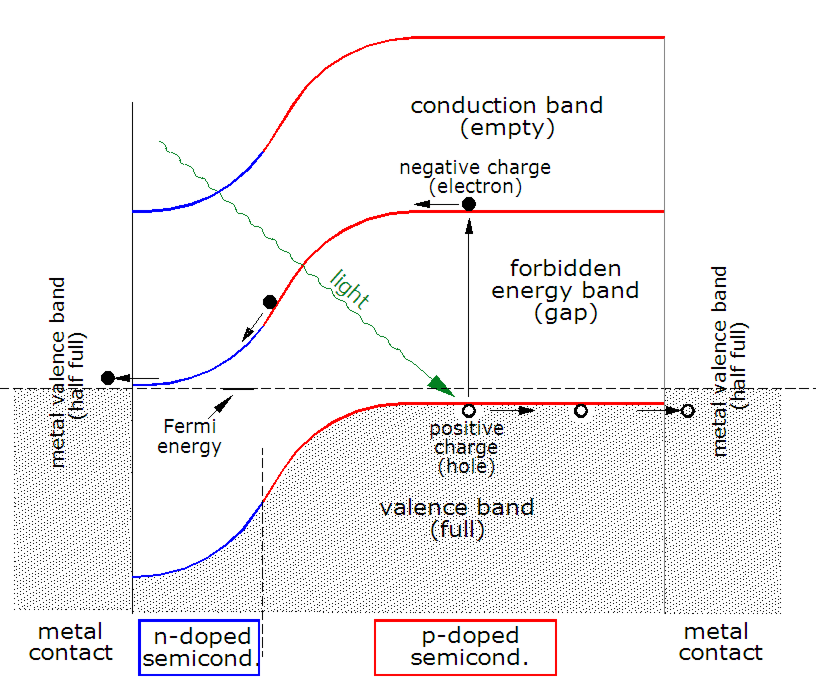
\includegraphics[width=\textwidth]{./Slike/PV-band-diagram}
 \caption{Band diagram of a solar cell~\cite{wiki:solar-cells}}
\label{fig:pv-band-diagram}
\end{figure}

The downside of solar generators is the constant changing of their power output. Fortunately, there are several methods to work around this shortcoming. One way to is to use supercapacitors~\cite{cap-wsn-ieee} to store the produced energy. Even so, with variable weather conditions, the cell is not always operating with its peak efficiency. The shift in its optimal power point can be seen in Figure~\ref{fig:pv-power-curve}. It is possible to offset this by using a system that dynamically adjusts the cell voltage to find the maximum power point~\cite{solar-mppt-ieee}. 

\begin{figure}
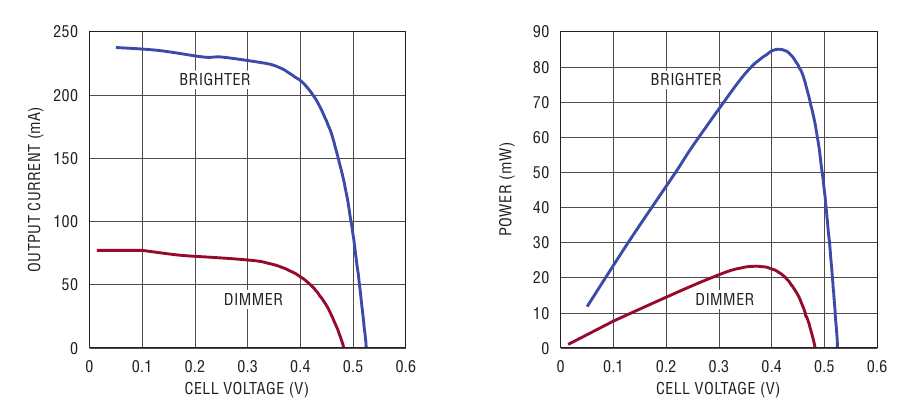
\includegraphics[width=\textwidth]{./Slike/PV-power-curve}
 \caption{Typical $I(V)$ and power curve of a 2x1 inch (13 cm$^2$) polycrystalline cell~\cite{Burgoine11}}
\label{fig:pv-power-curve}
\end{figure}


\section{\acl{TEG}}

Another source of energy in the environment is a temperature gradient. Using the Seebeck effect, it is possible to convert this difference in temperatures into electricity. This method has become very popular in the recent years, mostly due to their reliability and lower cost than photovoltaics. 

\acp{TEG} are typically made from a series of alternating N-doped and P-doped semiconductors, sandwiched between two ceramic plates~\cite{salerno10}. A schematic of their design can be seen in Figure~\ref{fig:teg-schematic}

\begin{figure}[h]
\subfigure{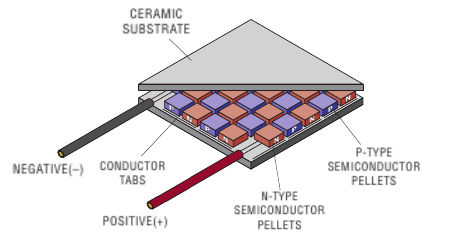
\includegraphics[height=100pt]{./Slike/TEG-shema}}
\subfigure{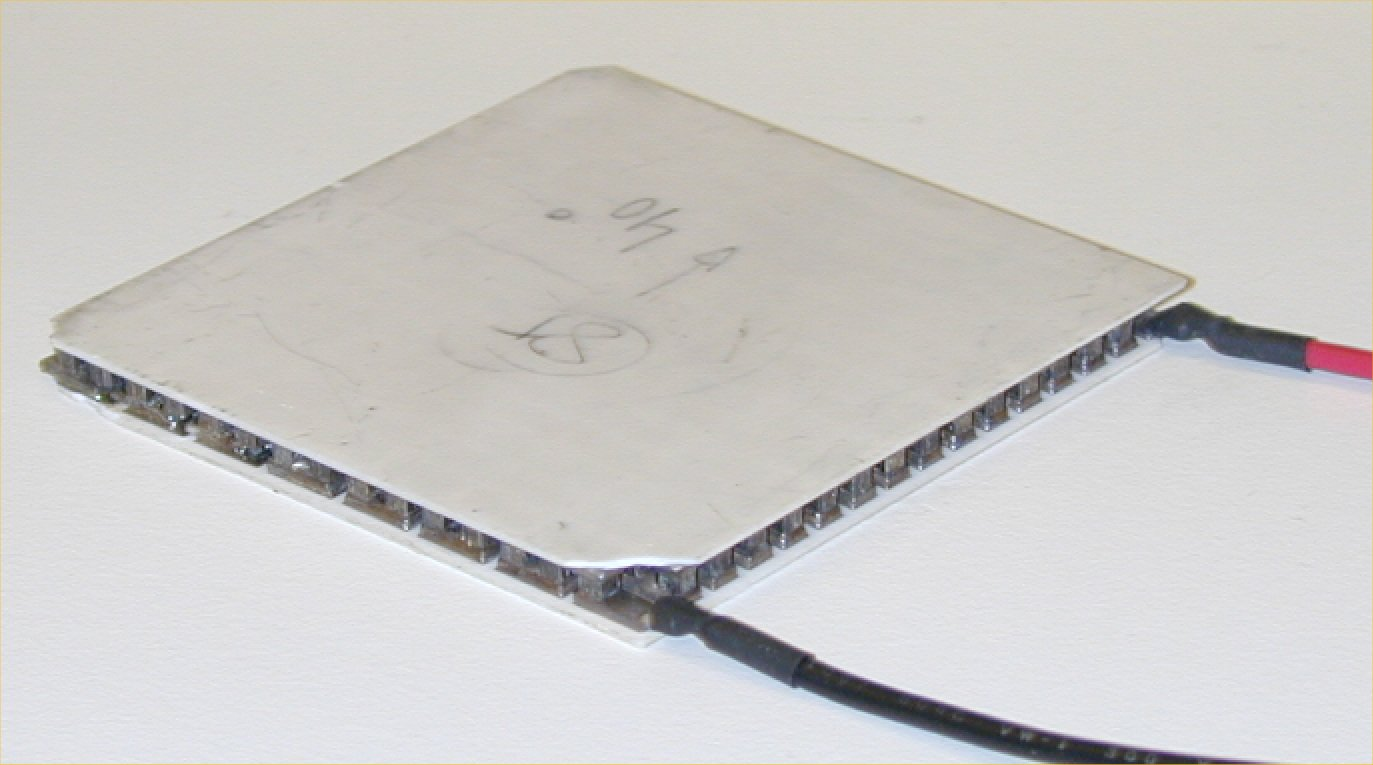
\includegraphics[height=100pt]{./Slike/TEG-slika}}
\caption{A schematic (left) and a photo (right) of a \ac{TEG} element~\cite{salerno10,wiki:teg}}
\label{fig:teg-schematic}
\end{figure}


\section{Piezoelectric generators}

The third most common form of \ac{EH} is generating power from the energy of motion. Vibrations are present especially in the vicinity of working machinery, but energy can also be produced from human activities, such as walking~\cite{piezo-shoe-ieee}. 

\section{Energy management and storage}

As mentioned above, electrical power from \ac{EH} generators can be very sporadic, and so can be the required load. Therefore, managing and storing the produced energy is very important. 

For energy storage, either batteries or ultracapacitors are used. Ultracapacitors, also known as Electric double-layer capacitors, are the newer technology, and are used where higher power density (as opposed to energy density) is required. En example of such a system is a wireless sensor node with its short spike of power consumption during transmission of data~\cite{cap-wsn-ieee}. Other advantages of supercapacitors include long life with no danger of overcharging or over-discharging and low internal resistance, while their main disadvantages are lowel energy density and high self-discharge rate~\cite{wiki:edlc}. 

\begin{figure}
\def\svgwidth{\textwidth}
 \input{./Slike/Supercapacitors_chart.pdf_tex}
\caption{Comparison of energy storage options~\cite{wiki:edlc}}
% Sem vzel iz Wikipedije, morda bi bilo prav citirati
\label{fig:storage-chart}
\end{figure}


\section{Conclusion}

\bibliography{harvesting}
\bibliographystyle{unsrt} 

\end{document}
